\section{Cloud Architektur}

Bei den Cloud Architekturen gibt es genau 3 verschiedene Rollen:
\begin{enumerate}
	\item \textbf{Provider:} bietet Cloud Produkte/Lösungen an
	\item \textbf{Konsumenten:} konsumieren Cloudlösungen
	\item \textbf{Klient:} nehmen Cloudlösungen (Anwendungen/Daten) in Anspruch
\end{enumerate}

\subsection{Konzeptuelle Sichtweise}

In diesem Abschnitt werden die Architekturen der einzelnen Kategorien von Cloudlösungen beschrieben.

\subsubsection{Konsumenten Sichtweise}

Wie in \textbf{Abbildung \ref{ConsumerView}} zu sehen, werden Ressourcen in Form von Clustersystemen vom Provider zur Verfügung gestellt.
Einzelne Klienten können über eine Netzwerkverbindung auf diese Ressourcen zeitgleich zugreifen. Der Provider kann außerdem den Pool
von Hardware Ressourcen verwalten, d.h. einzelne Hardware kann stillgelegt und ersetzt werden. Die Klienten werden nach dem stilllegen
auf andere Hardware Ressourcen weitergeleitet.
\todo{eventuell Rest hinzufügen}
\begin{figure}[H]
    \centering
	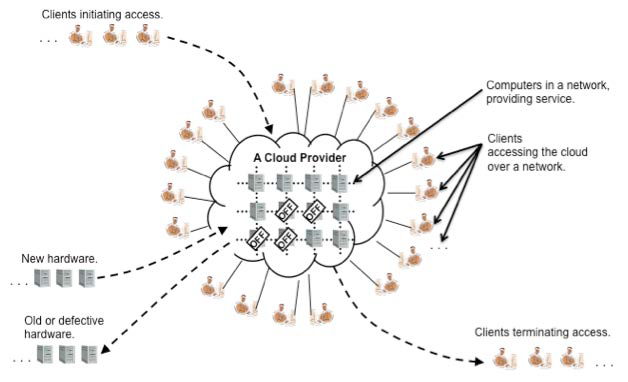
\includegraphics[width=0.4\textwidth]{Images/ConsumerView}
	\caption{Konsumenten Sichtweise \cite{Badger}}
	\label{ConsumerView}
\end{figure}


Alle Kategorien von Cloud-Computing können sogenannte Sicherheitsperimeter verwenden. Diese Regeln den Zugriff auf die Ressource.
In unseren Beispielen kann ein Klient, der sich außerhalb des Sicherheitsperimeter befindet, nur durch einen \glqq boundary controller\grqq
Zugriff zum Netzwerk erlangen.

\subsubsection{Lokale Private Cloud}

Wie in \textbf{Abbildung \ref{PrivateCloud}} zu sehen, befindet sich eine Private Cloud innerhalb der Organisation.
Klienten, die sich innerhalb des Sicherheitsperimeters befinden, können sich mit der Privaten Cloud verbinden. 
Klienten von außerhalb, können eine Verbindung durch den \glqq boundary controller\grqq aufbauen. Dieser Sicherheitsperimeter ist in diesem
Fall optional und wird von dem Konsumenten verwaltet.

\begin{figure}[H]
    \centering
	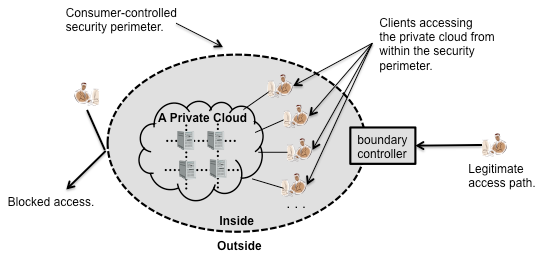
\includegraphics[width=0.4\textwidth]{Images/On-sitePrivateCloud}
	\caption{Private Cloud \cite{Badger}}
	\label{PrivateCloud}
\end{figure}

Die Verwaltung der Cloud wird vom Konsumenten übernommen. Dieser muss die Cloud so einstellen, dass die Arbeitslast zwischen verschiedenen
Maschinen verteilt werden kann, um die Ressourcen optimal nutzen zu können. Außerdem sollten redundante Kopien der Daten auf verschiedenen Maschinen 
gespeichert werden. Dies hat den Vorteil, dass bei einem Serverausfall der Klient auf eine andere Maschine weitergeleitet werden kann.
Außerdem muss der Konsument sicherstellen, dass wichtige Daten wie z.B. Lohnabrechnungen nicht von allen Klienten zugegriffen werden können,
da verschiedenen Daten auf einer Maschine verarbeitet werden können. Der Nachteil von Privaten Clouds ist, dass es hohe Anschaffungskosten, wie z.B. 
das Anschaffen von neuen Daten Zentren, gibt. Außerdem müssen bei z.B. steigenden Zugriffszahlen, neue Hardware vom Konsumenten bereitgestellt werden. 
Dies verringert Flexibilität des Konsumenten.

\subsubsection{Ausgelagerte Private Cloud}

Bei der ausgelagerten Privaten Cloud, wird die Cloud zu einem Provider verlagert. Dieser separiert das Organisationsnetzwerk
von seinem \glqq öffentlichen\grqq Netzwerk, wie in \textbf{Abbildung \ref{OutSourcedPrivateCloud}} zu sehen ist. Das Netzwerk wird vom Provider
durch einen Sicherheitsperimeter geschützt. Der Provider muss dabei sicherstellen, dass die Sicherheitsanforderungen des Konsumenten erfüllt werden. 
Der Konsument kann ebenfalls einen Sicherheitsperimeter in seiner Organisation installieren, um den Zugriff zur Cloud zu regeln.
Die beiden Perimeter werden dann durch einen Kommunikationskanal verbunden und Klienten können dann nur über diesen Kanal auf Daten der Cloud zugreifen.

\begin{figure}[H]
    \centering
	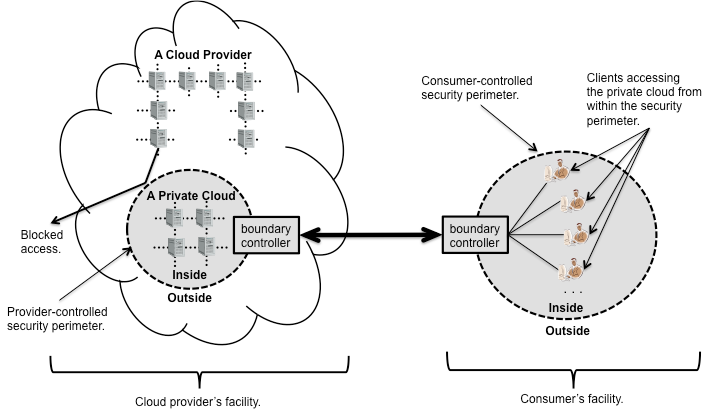
\includegraphics[width=0.4\textwidth]{Images/OutSourcedPrivateCloud}
	\caption{Ausgelagerte Private Cloud \cite{Badger}}
	\label{OutSourcedPrivateCloud}
\end{figure}

Der Konsument ist in diesem Fall von der Netzwerkverfügbarkeit und -geschwindigkeit des Providers abhängig, kann die Geschwindigkeit aber durch Sondertarife erhöhen.
Der Provider muss außerdem sicherstellen, dass die Arbeitslast auf den verschiedenen Maschinen innerhalb des Perimeters verteilt wird und sich die Daten 
nicht mit den Daten von anderen Organisationen, außerhalb des Perimeters, vermischen.
Der Vorteil dieser Architektur ist es, dass der Konsument keine eigenen Ressourcen mehr anschaffen muss und diese beim Provider mieten kann.
Eine Erhöhung der verfügbaren Ressourcen kann jedoch vom Provider nur manuell geschehen, sofern dieser über genug Ressourcen verfügt. 



\subsubsection{Lokale Community Cloud}

Bei der Lokalen Community Cloud teilen mehrere Organisationen ihre Ressourcen und Daten. Alle Organisation stellen und/oder konsumieren Cloud Services.
Dabei muss mindestens eine Organisation solche Services zur Verfügung stellen. Somit ist mindestens eine Organisation, sowohl Provider als auch Konsument.
Sollte jede Organisation einen Sicherheitsperimeter installieren, werden die einzelnen Organisationen durch Kommunikationskanäle zwischen den \glqq boundary controller\grqq verbunden.
Organisationen können außerdem einen weiteren Sicherheitsperimeter einrichten, um die lokalen Cloud Ressourcen von den lokalen Ressourcen zu trennen.

\begin{figure}[H]
    \centering
	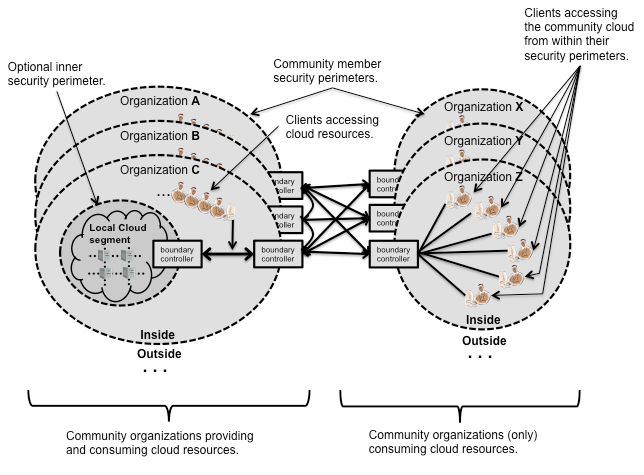
\includegraphics[width=0.4\textwidth]{Images/On-siteCommunityCloud}
	\caption{Lokale Community Cloud \cite{Badger}}
	\label{On-siteCommunityCloud}
\end{figure}

Für die Verwendung der lokalen Community Cloud wird eine komplexe Sicherheitsauthentifizierung benötigt. Jede Organisation der Community muss einen Zugriff bieten und erhalten.
Außerdem müssen die Kommunikationskanäle geschützt und bei der Verwendung des öffentliche Internet Kryptographie verwenden werden. Die einzelnen Kommunikationskanäle zwischen den Teilnehmern 
können verschiedene Level der Performance, Sicherheit und Zuverlässigkeit bereitstellen, abhängig von den Ansprüchen der Teilnehmenden Organisationen. Die Sicherheit der einzelnen Clouds hängt 
hierbei von den den Sicherheitsperimeter der einzelnen Organisationen ab. Ein großer Nachteil dieser Methode sind die hohen Kosten der einzelnen Provider, die Ressourcen 
anschaffen und Services konfigurieren müssen. Die Konsumenten hingegen zahlen nur die Mietkosten der für die Verwendungen der einzelnen Clouds. Ein weiterer Nachteil ist, dass 
die Ressourcen lokal bereitgestellt werden und somit limitiert sind. Wodurch die Flexibilität der einzelnen Organisationen sinkt.


\subsubsection{Ausgelagerte Community Cloud}

Bei der Ausgelagerten Community Cloud verhält es sich ähnlich zu der Ausgelagerten Privaten Cloud, wie in \textbf{Abbildung \ref{OutSourcedCommunityCloud}} zu sehen ist.
Um die Serverseitige Verantwortung kümmert sich hier der Provider, der ein Sicherheitsperimeter installiert und verwaltet. Dabei sorgt der Provider dafür, dass sich 
die Community Ressourcen und die Cloud Provider Ressourcen, die sich außerhalb des Perimeters befinden, nicht vermischen. Ein wesentlicher Unterschied zur Ausgelagerten Privaten Cloud
besteht darin, dass der Cloud Provider möglicherweise eine Freigaberichtlinie zwischen den teilnehmenden Unternehmen der Community Cloud durchsetzen muss. 
Um den Organisationen der Community Konsumenten eine Verbindung zur Cloud zu ermöglichen, müssen sichere Kommunikationskanäle zwischen den einzelnen Organisationen und 
dem Provider installiert werden. 

\begin{figure}[H]
    \centering
	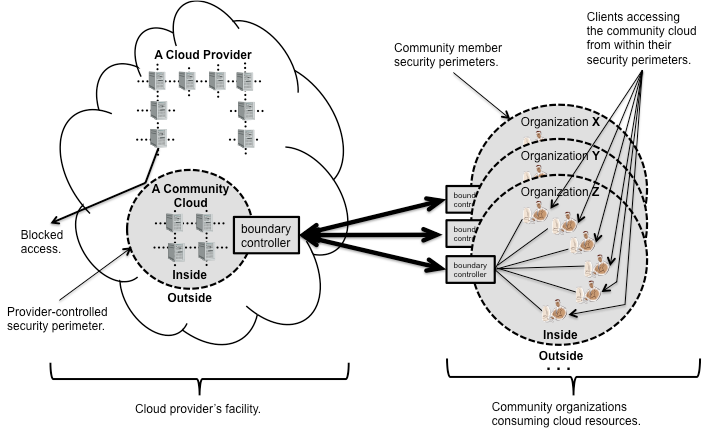
\includegraphics[width=0.4\textwidth]{Images/OutSourcedCommunityCloud}
	\caption{Ausgelagerte Community Cloud \cite{Badger}}
	\label{OutSourcedCommunityCloud}
\end{figure}


\subsubsection{Public Cloud}

Die Public Cloud, die in \textbf{Abbildung \ref{PublicCloud}} zu sehen ist, verhält sich recht ähnlich zu \textbf{Abbildung \ref{ConsumerView}}.
Außer das der Konsument einen eigenen Sicherheitsperimeter installiert, um den Zugriff zur Cloud zu regeln.

 
\begin{figure}[H]
    \centering
	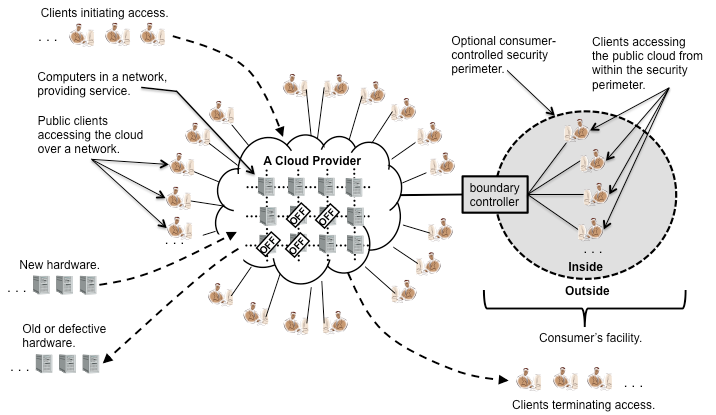
\includegraphics[width=0.4\textwidth]{Images/PublicCloud}
	\caption{Public Cloud \cite{Badger}}
	\label{PublicCloud}
\end{figure}

In diesem Szenario verbindet sich der Konsument über das öffentliche Internet, sodass die Verbindungsqualität und -zuverlässigkeit zur Cloud
von dem Internet Provider, dem DNS Server und der Router Infrastruktur abhängt. Die Arbeitslast oder Ressourcen eines Konsumenten können zu jeder Zeit
vom Provider migriert werden. Ein großer Vorteil der Public Cloud ist die Kosteneffizient, da Datenzentren an Standorten verwendet werden können, die für den Konsumenten am günstigen sind.
Ein Beispiel dafür wäre, das die Arbeitslast eines Deutschen Unternehmens in einem Deutschen Datenzentrum verarbeitet und somit die Performance verbessert wird (geringe Übertragungswege).
Dies wird aber meist nicht von Provider versichert. Die Arbeitslast kann an verschiedenen Standorten (Europa, USA, China usw.) verarbeitet werden, außer der Provider bietet eine
Standortbeschränkung an. Ein großes Problem der Public Cloud ist es, dass eine Maschine die Daten von mehreren Konsumenten verarbeiten kann und somit ein Sicherheitsrisiko entstehen kann.
Außerdem haben die Konsumenten keine Möglichkeit die Einsicht ihrer Daten zu überwachen oder eine Authentifizierung für ihre Daten einzurichten. Da große Anbieter meist eine Monitoring für die
Daten durchführen, um die Tatsächliche Datennutzung zu ermitteln und den Konsumenten diese dann in Rechnung zu stellen, ist diese Methode nicht für sensible oder wichtige Daten geeignet.
Außerdem kann der Konsument nie sicher sein, ob sein Daten auch gelöscht werden, wenn er den Vertrag kündigt. 
Ein großer Vorteil der Public Cloud ist die Uneingeschränktheit in Hinsicht des Standortes und der Größe. D.h. die Größe der zur Verfügung gestellten Ressourcen lässt sich 
meist \glqq uneingeschränkt\grqq erhöhen oder vermindern.

Bekannte Public Cloud Provider sind Amazon Web Services (AWS) und Microsoft Azure. 


% \subsubsection{Hybrid Cloud}
% Eine Hybrid Cloud besteht aus mindestens zwei oder mehreren Privaten, Community oder Public Clouds.
% \begin{figure}[H]
%     \centering
% 	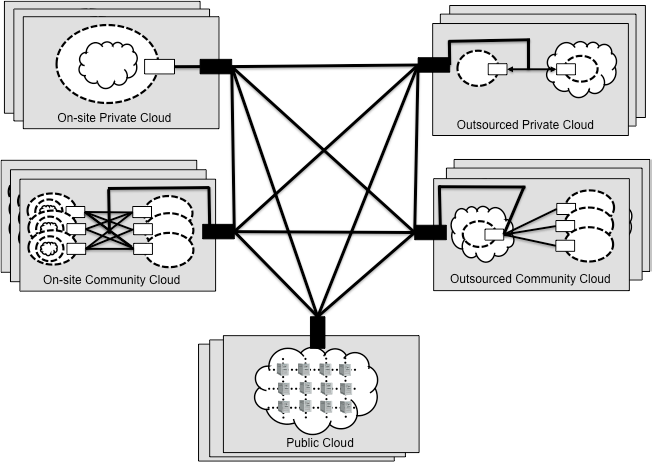
\includegraphics[width=0.4\textwidth]{Images/HybridCloud}
% 	\caption{Hybrid Cloud \cite{Badger}}
% 	\label{HybridCloud}
% \end{figure}

\subsection{Architekturen der Dienstmodelle}

In diesem Abschnitt werden die drei Dienstmodelle die Public Cloud Provider ihren Kunden (Konsumenten) anbieten, 

\subsubsection{SaaS}

\begin{figure}[H]
    \centering
	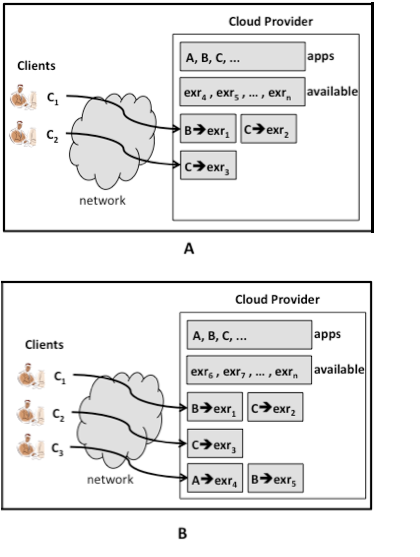
\includegraphics[width=0.4\textwidth]{Images/SaaSInteraction}
	\caption{SaaS Interaktion \cite{Badger}}
	\label{SaaSInteraction}
\end{figure}


aaa
\begin{figure}[H]
    \centering
	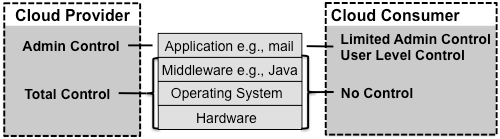
\includegraphics[width=0.4\textwidth]{Images/SaaSControl}
	\caption{SaaS Kontrollverteilung \cite{Badger}}
	\label{SaaSControl}
\end{figure}

aaaaaa
\begin{figure}[H]
    \centering
	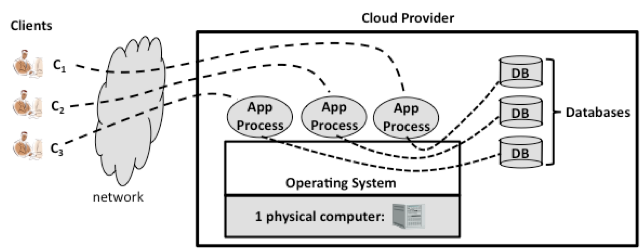
\includegraphics[width=0.4\textwidth]{Images/SaaSM1}
	\caption{Möglichkeit 1 \cite{Badger}}
	\label{SaaSM1}
\end{figure}

aaa

\begin{figure}[H]
    \centering
	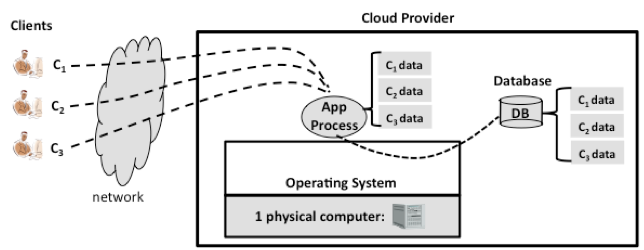
\includegraphics[width=0.4\textwidth]{Images/SaaSM2}
	\caption{Möglichkeit 2 \cite{Badger}}
	\label{SaaSM2}
\end{figure}

\subsubsection{Paas}
aaa

\begin{figure}[H]
    \centering
	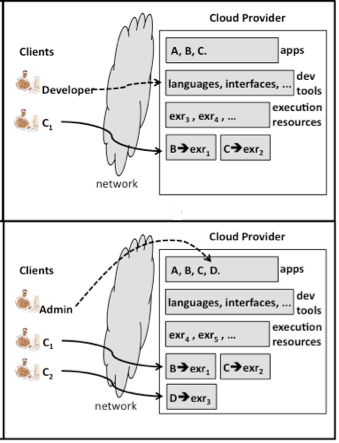
\includegraphics[width=0.4\textwidth]{Images/PaaSInteraction}
	\caption{PaaS Interaktion \cite{Badger}}
	\label{PaaSInteration}
\end{figure}

aaaaaa
\begin{figure}[H]
    \centering
	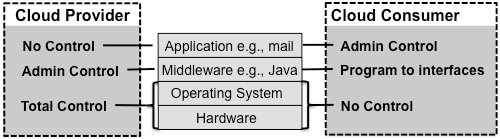
\includegraphics[width=0.4\textwidth]{Images/PaaSControl}
	\caption{PaaS Kontrollverteilung \cite{Badger}}
	\label{PaaSControl}
\end{figure}

\subsubsection{IaaS}
aaa
\begin{figure}[H]
    \centering
	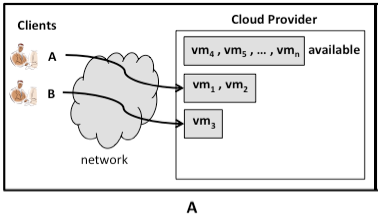
\includegraphics[width=0.4\textwidth]{Images/IaaSInteraction}
	\caption{IaaS Interaktion \cite{Badger}}
	\label{IaaSInteraction}
\end{figure}

aaa
\begin{figure}[H]
    \centering
	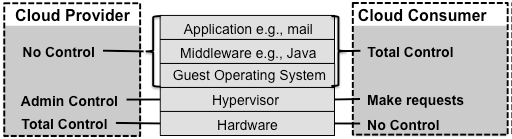
\includegraphics[width=0.4\textwidth]{Images/IaaSControl}
	\caption{IaaS Kontrollverteilung \cite{Badger}}
	\label{IaaSControl}
\end{figure}

\subsection{Logische Sichtweise}
aaaaaaaaa
\begin{figure}[H]
    \centering
	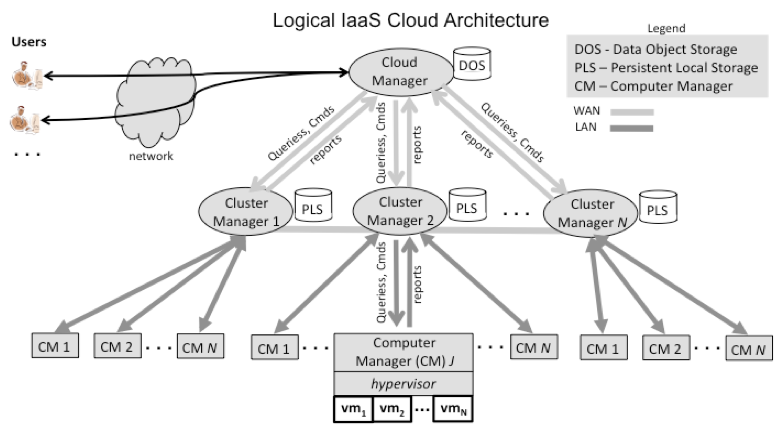
\includegraphics[width=0.4\textwidth]{Images/IaaSLogic}
	\caption{IaaS Logische Sichtweise \cite{Badger}}
	\label{IaaSLogic}
\end{figure}

% \subsection{Management}
%\pagebreak